\documentclass{beamer}
\usepackage{amsmath}
\usepackage[english]{babel} %set language; note: after changing this, you need to delete all auxiliary files to recompile
\usepackage[utf8]{inputenc} %define file encoding; latin1 is the other often used option
\usepackage{csquotes} % provides context sensitive quotation facilities
\usepackage{graphicx} %allows for inserting figures
\usepackage{booktabs} % for table formatting without vertical lines
\usepackage{textcomp} % allow for example using the Euro sign with \texteuro
\usepackage{stackengine}
\usepackage{wasysym}
\usepackage{tikzsymbols}
\usepackage{textcomp}
\newcommand{\bubblethis}[2]{
        \tikz[remember picture,baseline]{\node[anchor=base,inner sep=0,outer sep=0]%
        (#1) {\underline{#1}};\node[overlay,cloud callout,callout relative pointer={(0.2cm,-0.7cm)},%
        aspect=2.5,fill=yellow!90] at ($(#1.north)+(-0.5cm,1.6cm)$) {#2};}%
    }%
\tikzset{face/.style={shape=circle,minimum size=4ex,shading=radial,outer sep=0pt,
        inner color=white!50!yellow,outer color= yellow!70!orange}}
%% Some commands to make the code easier
\newcommand{\emoticon}[1][]{%
  \node[face,#1] (emoticon) {};
  %% The eyes are fixed.
  \draw[fill=white] (-1ex,0ex) ..controls (-0.5ex,0.2ex)and(0.5ex,0.2ex)..
        (1ex,0.0ex) ..controls ( 1.5ex,1.5ex)and( 0.2ex,1.7ex)..
        (0ex,0.4ex) ..controls (-0.2ex,1.7ex)and(-1.5ex,1.5ex)..
        (-1ex,0ex)--cycle;}
\newcommand{\pupils}{
  %% standard pupils
  \fill[shift={(0.5ex,0.5ex)},rotate=80] 
       (0,0) ellipse (0.3ex and 0.15ex);
  \fill[shift={(-0.5ex,0.5ex)},rotate=100] 
       (0,0) ellipse (0.3ex and 0.15ex);}

\newcommand{\emoticonname}[1]{
  \node[below=1ex of emoticon,font=\footnotesize,
        minimum width=4cm]{#1};}
\usepackage{scalerel}
\usetikzlibrary{positioning}
\usepackage{xcolor,amssymb}
\newcommand\dangersignb[1][2ex]{%
  \scaleto{\stackengine{0.3pt}{\scalebox{1.1}[.9]{%
  \color{red}$\blacktriangle$}}{\tiny\bfseries !}{O}{c}{F}{F}{L}}{#1}%
}
\newcommand\dangersignw[1][2ex]{%
  \scaleto{\stackengine{0.3pt}{\scalebox{1.1}[.9]{%
  \color{red}$\blacktriangle$}}{\color{white}\tiny\bfseries !}{O}{c}{F}{F}{L}}{#1}%
}
\usepackage{fontawesome} % Social Icons
\usepackage{epstopdf} % allow embedding eps-figures
\usepackage{tikz} % allows drawing figures
\usepackage{amsmath,amssymb,amsthm} %advanced math facilities
\usepackage{lmodern} %uses font that support italic and bold at the same time
\usepackage{hyperref}
\usepackage{tikz}
\usepackage{tcolorbox}

\usefonttheme[onlymath]{serif} %set math font to serif ones

\definecolor{beamerblue}{rgb}{0.2,0.2,0.7} %define beamerblue color for later use

%%% defines highlight command to set text blue
\newcommand{\highlight}[1]{{\color{blue}{#1}}}


%%%%%%% commands defining backup slides so that frame numbering is correct

\newcommand{\backupbegin}{
   \newcounter{framenumberappendix}
   \setcounter{framenumberappendix}{\value{framenumber}}
}
\newcommand{\backupend}{
   \addtocounter{framenumberappendix}{-\value{framenumber}}
   \addtocounter{framenumber}{\value{framenumberappendix}}
}

%%%% end of defining backup slides

%Specify figure caption, see also http://tex.stackexchange.com/questions/155738/caption-package-not-working-with-beamer
\setbeamertemplate{caption}{\insertcaption} %redefines caption to remove label "Figure".
%\setbeamerfont{caption}{size=\scriptsize,shape=\itshape,series=\bfseries} %sets figure  caption bold and italic and makes it smaller

\newtcolorbox{boxA}{
    fontupper = \bf,
    boxrule = 1.5pt,
    colframe = black % frame color
}

\usetheme{Boadilla}

% --------------------
% Overall information
% --------------------
\title[Economía I]{Economía I \vspace{4mm}
\\ Magistral 19: Introducción a la Macro}
\date{}
\author[Riottini]{Riottini Franco}
\vspace{0.4cm}
\institute[]{Universidad de San Andrés}

\begin{document}

\begin{frame}
\titlepage
\centering


\includegraphics[scale=0.2]{../Figures/logoUDESA.jpg} 
\end{frame}

\begin{frame}{Las grandes preguntas de la macroeconomía}
    \begin{itemize}
        \item ¿Por qué la economía vive ciclos de expansión y de recesión?
        \item ¿Qué determina el nivel agregado de producción?
        \item ¿Qué determina el crecimiento de largo plazo?
    \end{itemize} \pause
    
    \begin{boxA}
        El PBI se define como el valor de mercado del conjunto de bienes y servicios finales que se produce en una economía en un
        determinado período de tiempo.
    \end{boxA}
\end{frame}

\begin{frame}{Flujo Circular de la Renta (cerrado)}
    \begin{figure} [H]   
        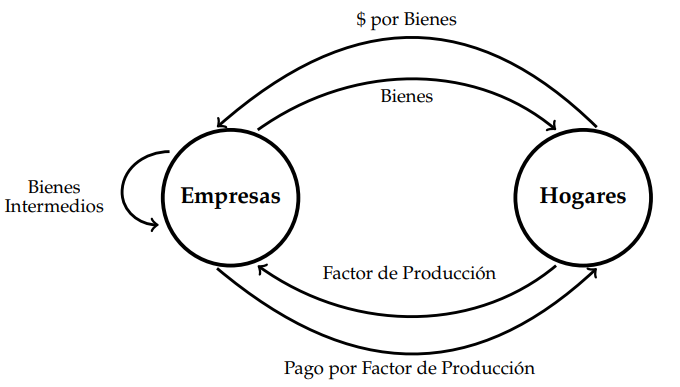
\includegraphics[scale=0.75]{../Figures/C29.1.png}
    \end{figure}
\end{frame}

\begin{frame}{PBI Nominal y Real}
    \begin{itemize}
        \item Considerar variables a \textit{valor de mercado} implica hacerlo a su precio\dots
        \item El PBI entonces es la suma de los bienes finales producidos a los precios de cada momento:
        \begin{equation*}
            PBI_{\text{NOMINAL}}^t = p_1^t q_1^t + p_2^t q_2^t + \cdots + p_N^t q_N^t.
        \end{equation*}
        \item Pero los precios cambian, por lo que el PBI nominal no es una buena medida de la producción real\dots
        \item Al PBI real lo vamos a definir como la suma de los bienes finales producidos en un año, pero valuados a los precios de un año base:
        \begin{align*}
            PBI_{\text{NOMINAL}}^i &= p_1^i q_1^i + p_2^i q_2^i + \cdots + p_N^i q_N^i \\
            PBI_{\text{NOMINAL}}^j &= p_1^j q_1^j + p_2^j q_2^j + \cdots + p_N^j q_N^j
        \end{align*}
        \begin{align*}
            PBI_{\text{REAL}}^i &= p_1^b q_1^i + p_2^b q_2^i + \cdots + p_N^b q_N^i \\
            PBI_{\text{REAL}}^j &= p_1^b q_1^j + p_2^b q_2^j + \cdots + p_N^b q_N^j
        \end{align*}
    \end{itemize}
\end{frame}

\begin{frame}{Componentes del PBI}
    \begin{itemize}
        \item Por el lado de la oferta:
        \begin{boxA}
            Llamamos PBI por el \textit{lado de la oferta} a la segmentación de
            los bienes y servicios finales según qué sectores los producen
        \end{boxA}
        \item Por el lado de la demanda:
        \begin{itemize}
            \item Consumo
            \item Inversión
            \item Gasto del gobierno
            \item Exportaciones Netas
            \item Cambio en los inventarios
        \end{itemize}
    \end{itemize}
    \begin{equation*}
        Y = C + I + G + X - M + \Delta \text{Inventarios}
    \end{equation*}
\end{frame}

% \begin{frame}{Flujo Circular de la Renta (abierto)}
%     \begin{figure} [H]   
%         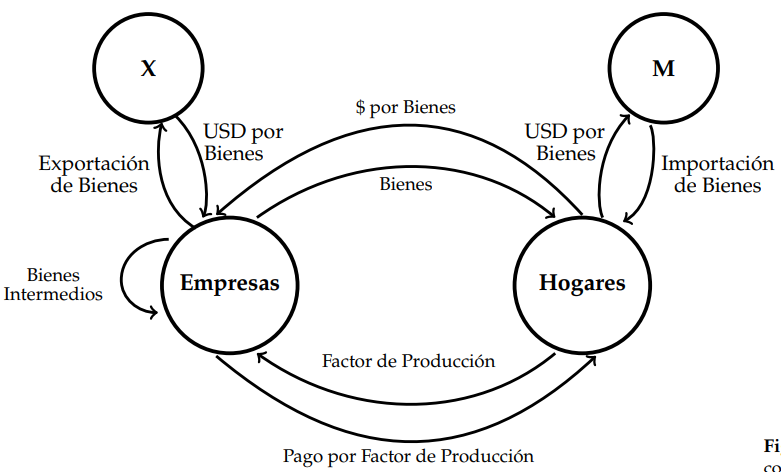
\includegraphics[scale=0.75]{../Figures/C29.4.png}
%     \end{figure}
% \end{frame}

\begin{frame}{Ciclos Económicos}
    \begin{itemize}
        \item Las fluctuaciones económicas de corto plazo nos interesan particularmente porque son el foco de la política económica.
        \item \textit{Políticas de Estabilización}: Políticas que buscan reducir la volatilidad de la economía.
        \item Los períodos de expansión y los períodos de contracción económica se conocen como \textbf{ciclo económico}.
        \begin{boxA}
            Decimos que la economía entra en una recesión si cae durante dos trimestres consecutivos, y
            decimos que sale de ella si tiene dos trimestres seguidos de crecimiento.
        \end{boxA}
        \item A una recesión abrupta las solemos denominar \textbf{depresión o crisis}.
    \end{itemize}
\end{frame}

\begin{frame}{El ciclo económico}
    \begin{figure} [H]   
        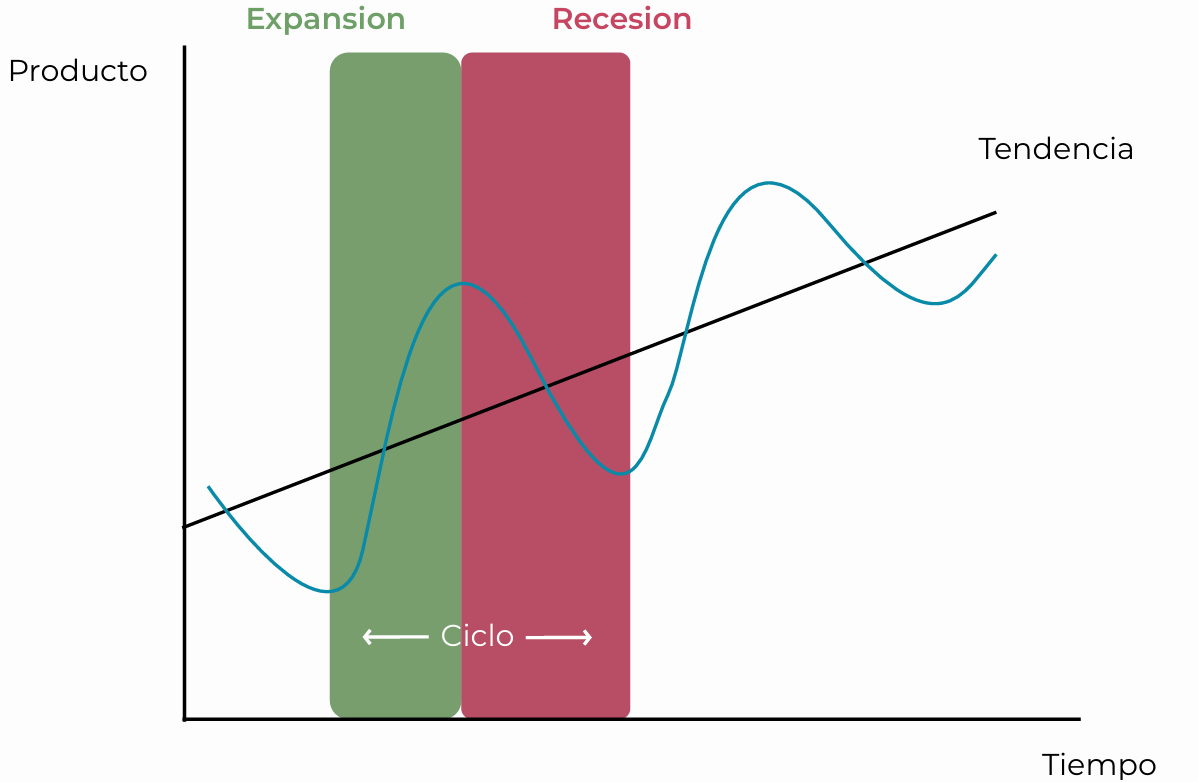
\includegraphics[width=12cm]{../Figures/32.7.png}
    \end{figure}
\end{frame}

\begin{frame}{Ciclos en el PBI en EEUU}

\centering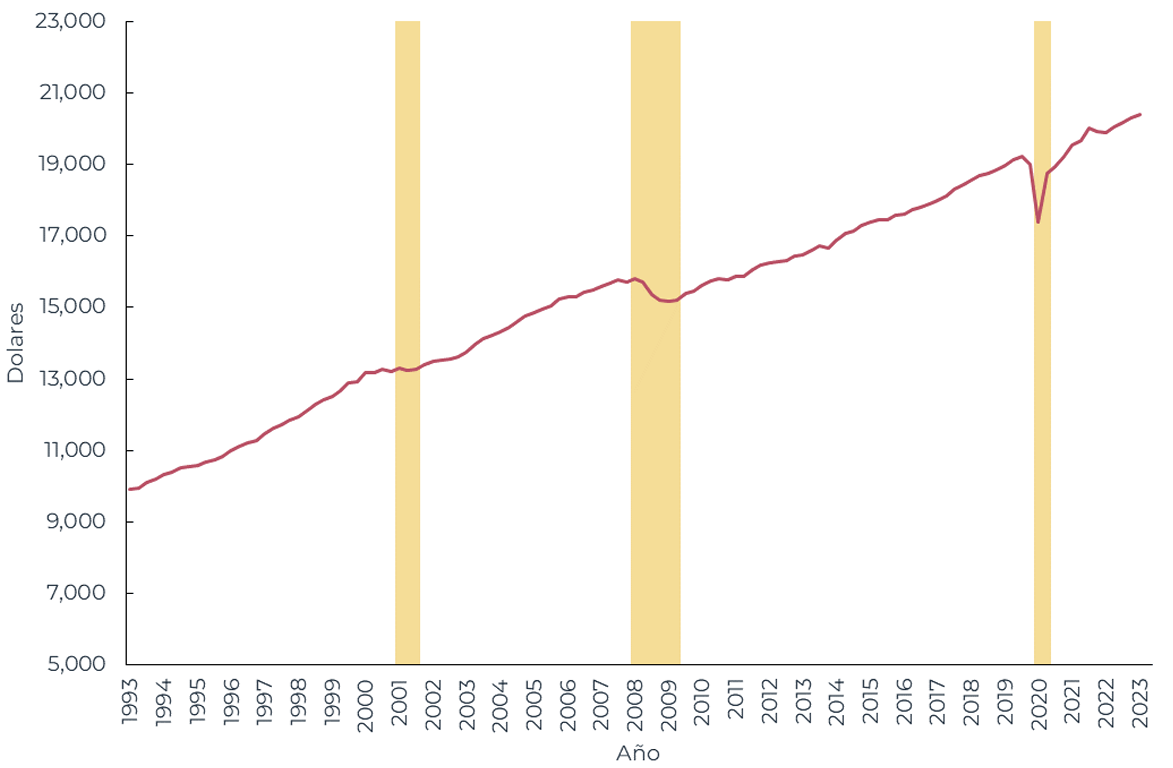
\includegraphics[width=12cm]{../Figures/32.8.png}\

\end{frame}

\begin{frame}{Ciclos en el PBI en Argentina}

\centering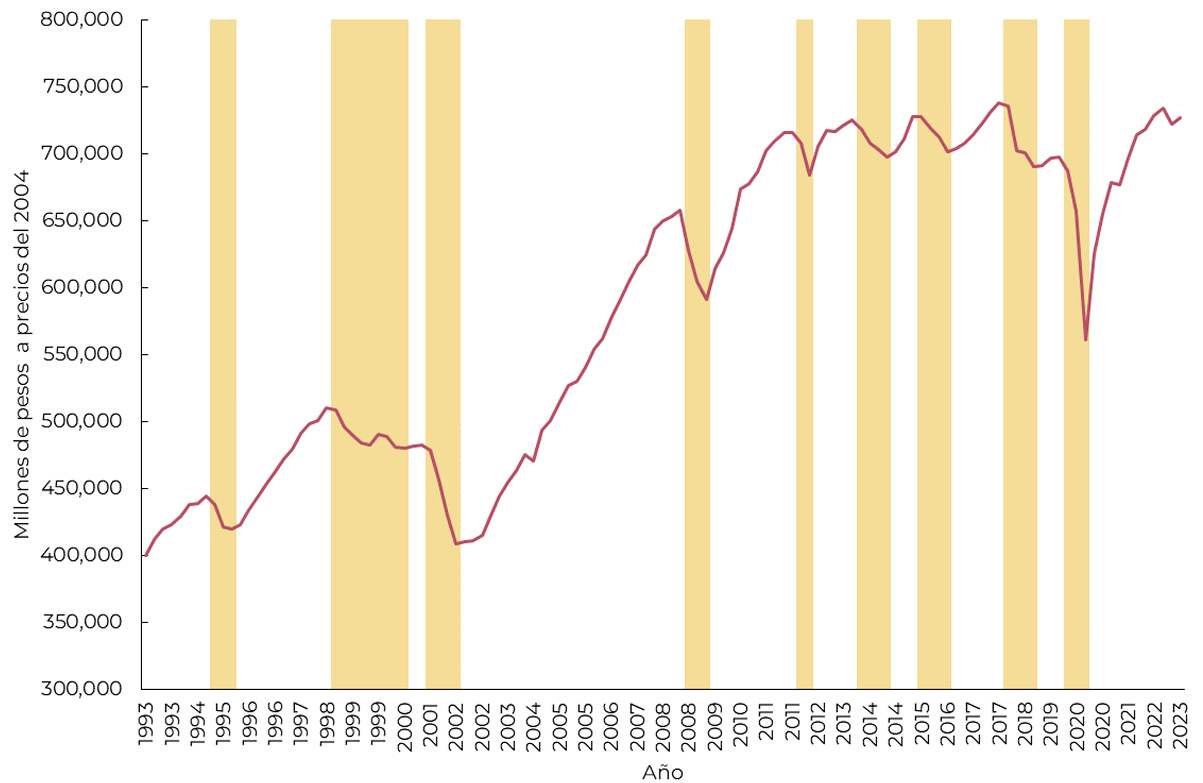
\includegraphics[width=12cm]{../Figures/32.9.png}\

\end{frame}

\begin{frame}{Ciclos Económicos comparados}

    \centering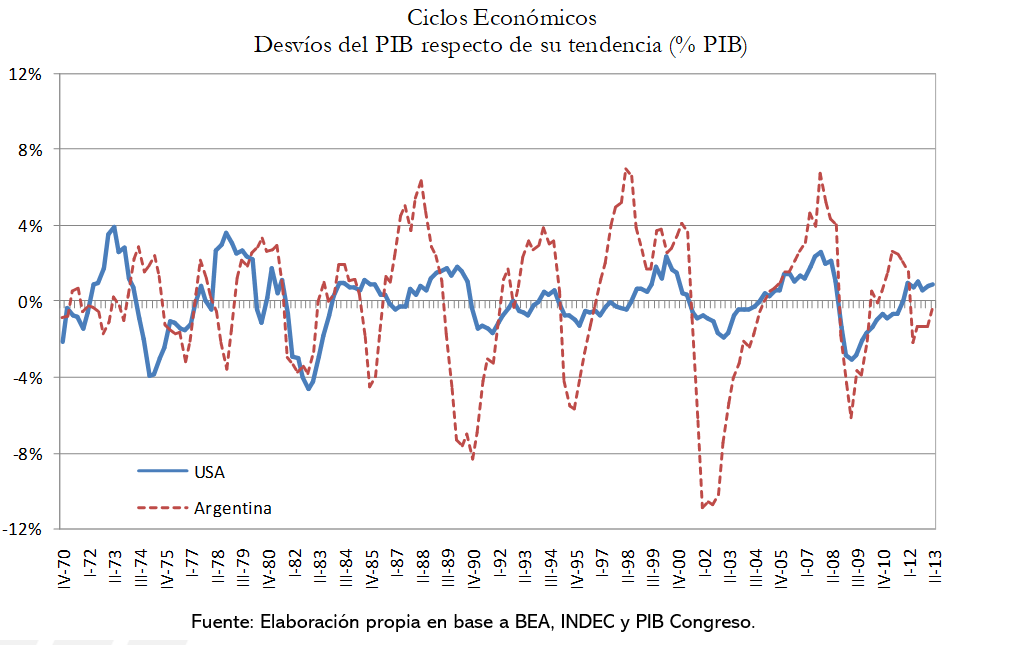
\includegraphics[width=12cm]{../Figures/P12.png}
    
\end{frame}

\begin{frame}{Estimando el ciclo}

    \centering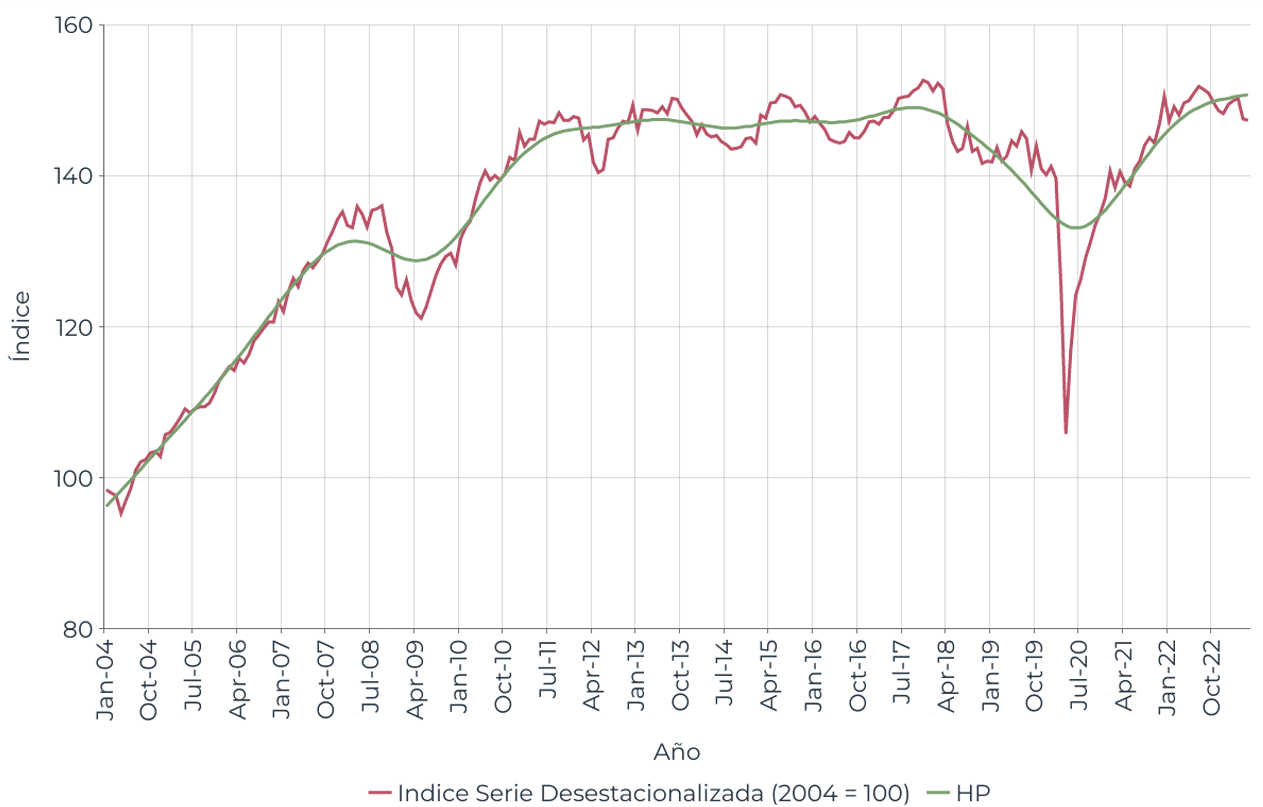
\includegraphics[width=12cm]{../Figures/32.13.png}
    
\end{frame}

\begin{frame}{Datos con estacionalidad vs. desestacionalizados}

\centering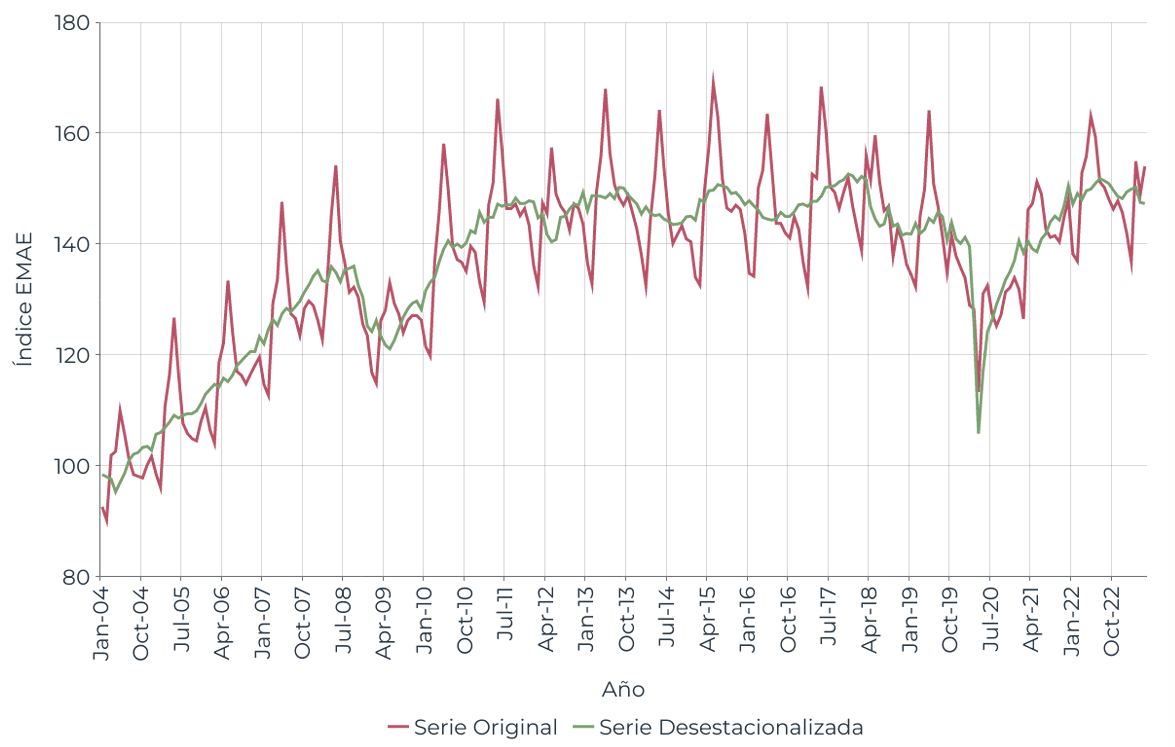
\includegraphics[width=11cm]{../Figures/32.14.png}

\end{frame}

\begin{frame}{Arrastre estadístico}
    \centering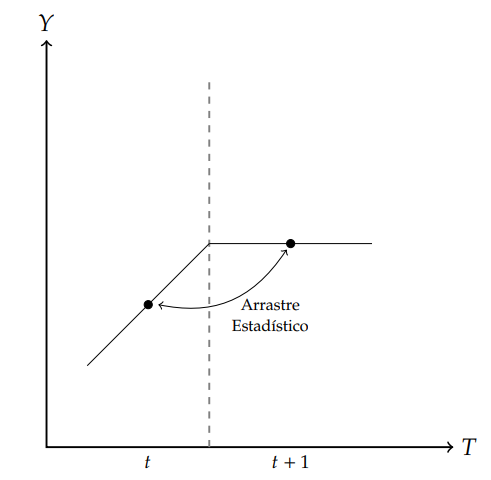
\includegraphics[width=8cm]{../Figures/C32.16.png}
\end{frame}

\begin{frame}{Evolución reciente del nivel de actividad}

    \centering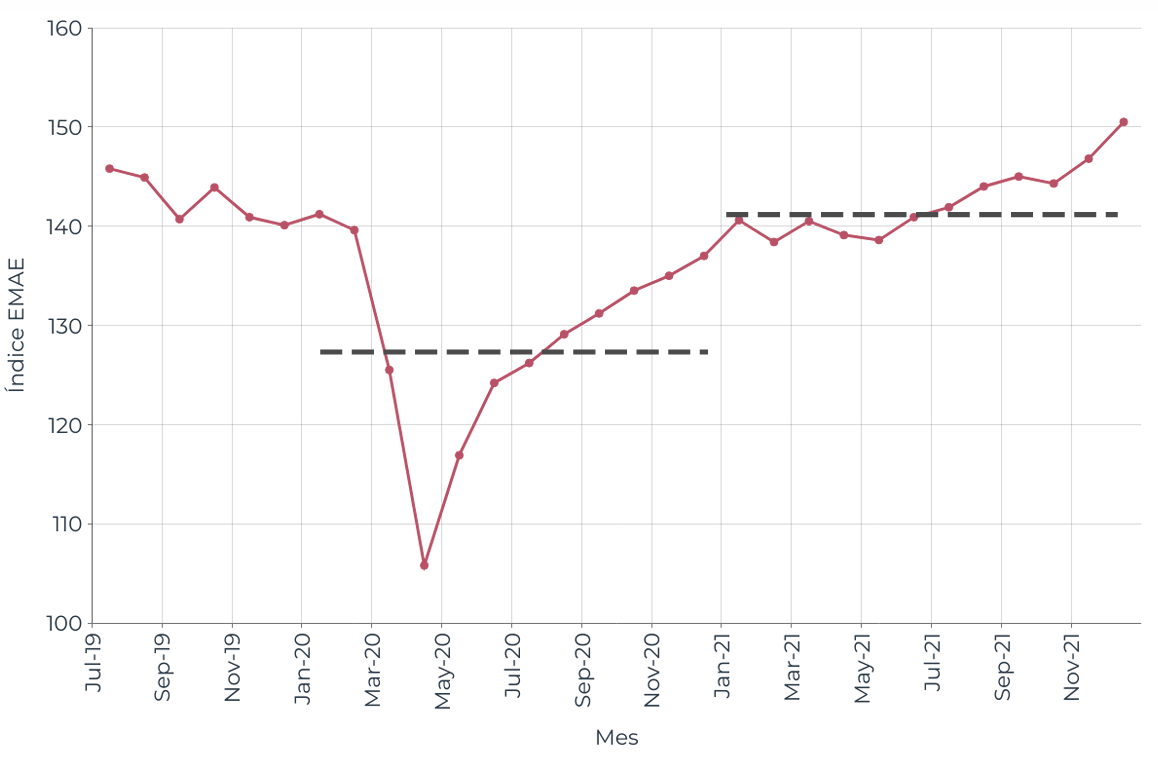
\includegraphics[width=11cm]{../Figures/32.16.png}

\end{frame}

\end{document}